\chapter[Processo de Engenharia de Requisitos]{Processo de Engenharia de Requisitos}
\label{chap:processo}
	Como retratado no Capítulo \ref{chap:justificativa} (\nameref{chap:justificativa}), a abordagem adotada pelo grupo para o desenvolvimento do projeto foi a adaptativa, ou ágil. De forma análoga à abordagem, referenciado por um estudo preciso do SAFe, resolveu-se realizar uma adaptação do \emph{framework}, desenhando um processo próprio de Engenharia de Requisitos.
	\\ \indent A seguir, na Seção \ref{sec:processo_safe} (\nameref{sec:processo_safe}), é descrito de forma genérica o SAFe, principal referência para a construção do processo de Engenharia de Requisitos proposto.
	\\ \indent Na Seção \ref{sec:processo_papeis} (\nameref{sec:processo_papeis}) é descrito os papéis atribuídos no contexto do projeto.
	\\ \indent Na Seção \ref{sec:processo_diagrama} (\nameref{sec:processo_diagrama}) é descrito o modelo do processo de Engenharia de Requisitos proposto para o contexto do projeto.
	\\ \indent Na Seção \ref{sec:processo_atividades} (\nameref{sec:processo_atividades}) é definido minuciosamente cada atividade presente no processo de Engenharia de Requisitos proposto.

	\newpage

	\begin{landscape}
		\section[\emph{Scaled Agile Framework}]{\emph{Scaled Agile Framework}}
		\label{sec:processo_safe}
			\begin{figure}[h]
				\centering
				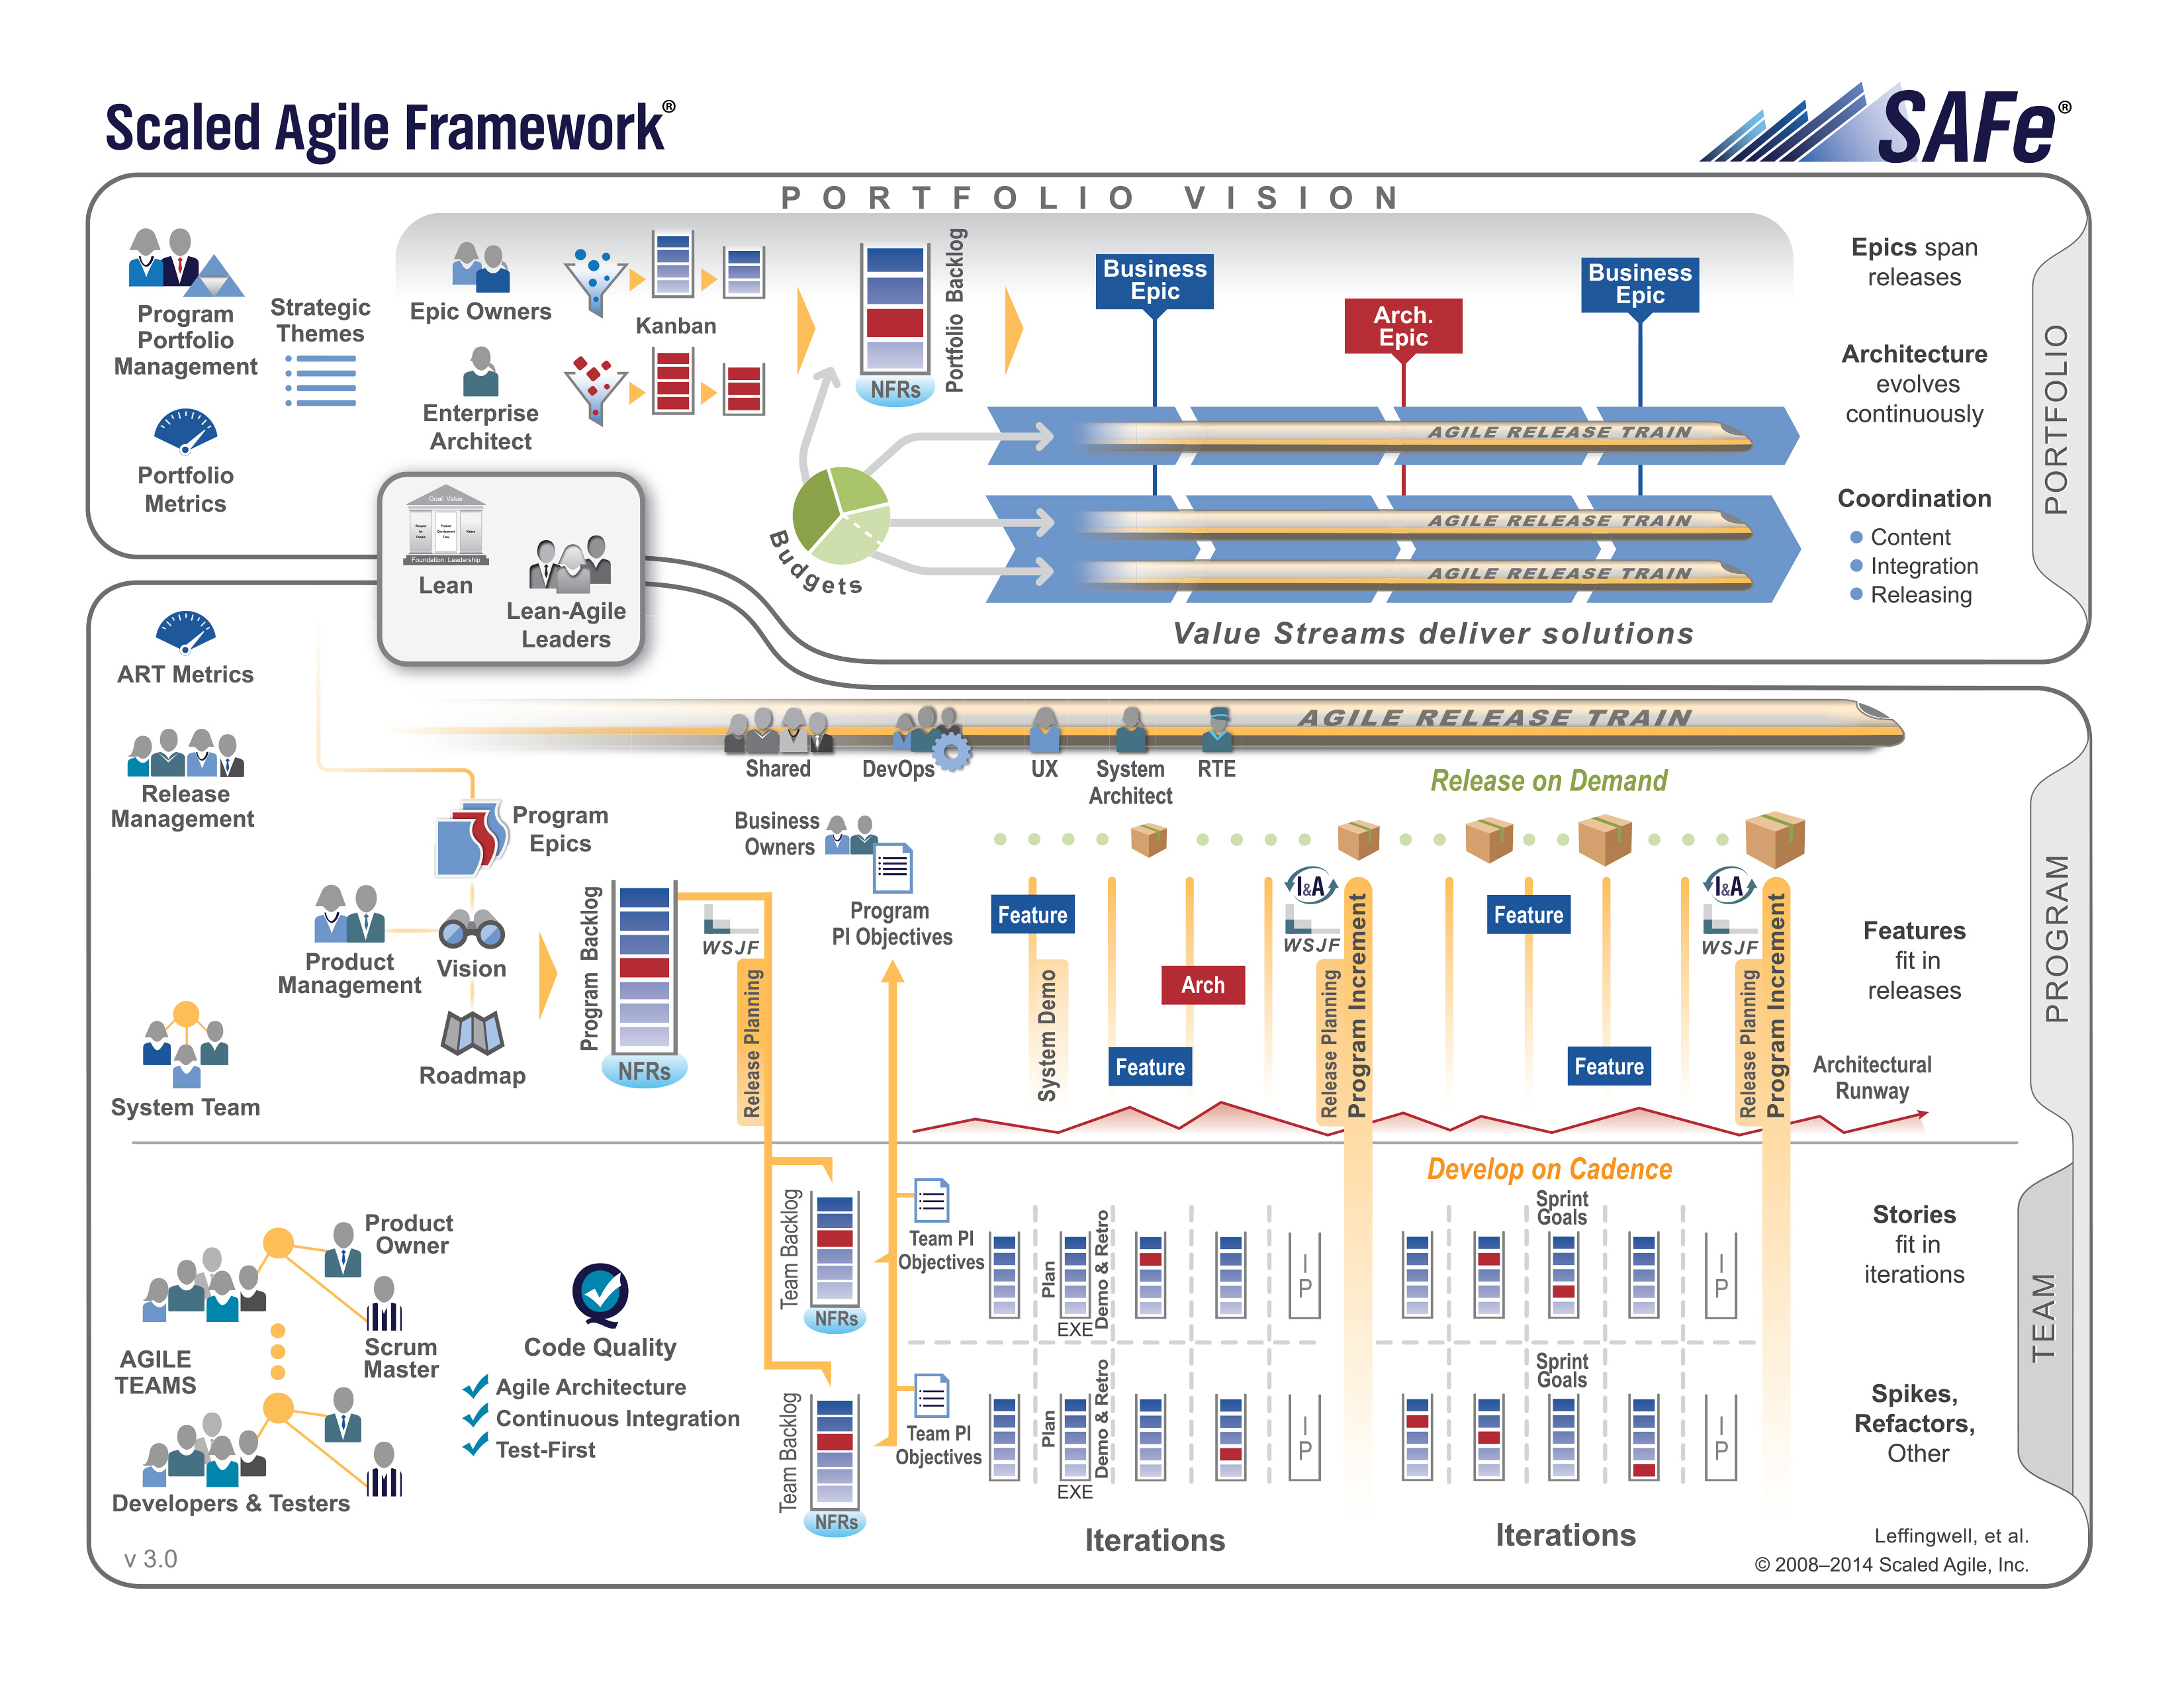
\includegraphics[scale=0.142]{safe}
				\caption[\emph{Scaled Agile Framework}]{Visão Geral do SAFe - \emph{Scaled Agile Framework} \cite{safe}.}
				\label{fig:modelo_processo}
			\end{figure}
	\end{landscape}

		\subsection[Nível de Portfólio]{Nível de Portfólio}
		\label{subsec:processo_safe_portfolio}
			No nível de portfólio, destaca-se os seguintes elementos:
			\begin{itemize}
				\item{\textbf{Temas de Investimento}: Representam um conjunto de iniciativas que irão dirigir os investimentos, em sistemas, produtos, aplicações e serviços;}
				\item{\textbf{Épicos}: São iniciativas de desenvolvimento em larga escala que irão gerar a entrega de novos produtos, soluções ou serviços para o cliente;}
				\item{\textbf{Arquitetura}: São iniciativas arquiteturais que visam dar conta da compatibilização tecnológica entre as soluções atuais e futuras.}
			\end{itemize}

		\subsection[Nível de Programa]{Nível de Programa}
		\label{subsec:processo_safe_programa}
			No nível de programa, destaca-se os seguintes elementos:
			\begin{itemize}
				\item{\textbf{\emph{Roadmap}}: Consiste em uma série de releases planejadas, com suas datas, features e priorizações;}
				\item{\textbf{\emph{Features}}: Serviços providos pelo sistema que atendem às necessidades dos \emph{Stakeholders}. São itens do \emph{Backlog} do programa;}
				\item{\textbf{\emph{Product Management}}: Responsável pela definição das features a nível de programa;}
				\item{\textbf{Requisitos Não-Funcionais}: Restrições ou condições que devem ser atendidas na construção da solução.}
			\end{itemize}

		\subsection[Nível de Time]{Nível de Time}
		\label{subsec:processo_safe_time}
			No nível de time, destaca-se os seguintes elementos:
			\begin{itemize}
				\item{\textbf{Scrum \emph{Master}}: Facilita a atuação do time para atingir seus objetivos. Lidera os esforços de melhoria contínua. Faz cumprir regras do processo ágil;}
				\item{\textbf{\emph{Product Owner}}: Trabalha com o gerente de produto, analistas de negócio, clientes e outros \emph{Stakeholders} para determinar os requisitos;}
				\item{\textbf{\emph{User Stories}}: Pequena declaração de intenção que descreve algo de necessário que o sistema deverá fazer para o usuário;}
				\item{\textbf{Iterações}: São pequenas, possuem tempo fixo. Entregam incrementos de software que agregam valor ao cliente.}
			\end{itemize}

	\section[Papéis]{Papéis}
	\label{sec:processo_papeis}
		Para o contexto da disciplina de Requisitos de \emph{Software}, levando em consideração a abordagem adaptativa, bem como particularidades do SAFe, os seguintes papéis foram discutidos e atribuidos:

		\subsection[Nível de Time]{Nível de Time}
		\label{subsec:processo_papeis_time}
			\begin{itemize}
				\item{\textbf{\emph{Product Owner}}: Grupo da disciplina de Modelagem de Processos, professor orientador;}
				\item{\textbf{\emph{Scrum Master}}: Monitores das Disciplinas;}
				\item{\textbf{\emph{Developers \& Testers} (Desenvolvedores e Testadores de Requisitos)}: Grupo da disciplina de Requisitos de \emph{Software}.}
			\end{itemize}

		\subsection[Nível de Programa]{Nível de Programa}
		\label{subsec:processo_papeis_programa}
			\begin{itemize}
				\item{\textbf{\emph{Product Management}}: Responsabilidade de todo o grupo da disciplina de Requisitos de \emph{Software}.}
			\end{itemize}

		\subsection[Nível de Portfólio]{Nível de Portfólio}
		\label{subsec:processo_papeis_programa}
			\begin{itemize}
				\item{\textbf{\emph{Epic Owner}}: O papel será executado uma vez pelo time da disciplina de Requisitos de \emph{Software}.}
			\end{itemize}

	\begin{landscape}
		\section[Modelo do Processo de Engenharia de Requisitos]{Modelo do Processo de Engenharia de Requisitos}
		\label{sec:processo_diagrama}
			\begin{figure}[h]
				\centering
				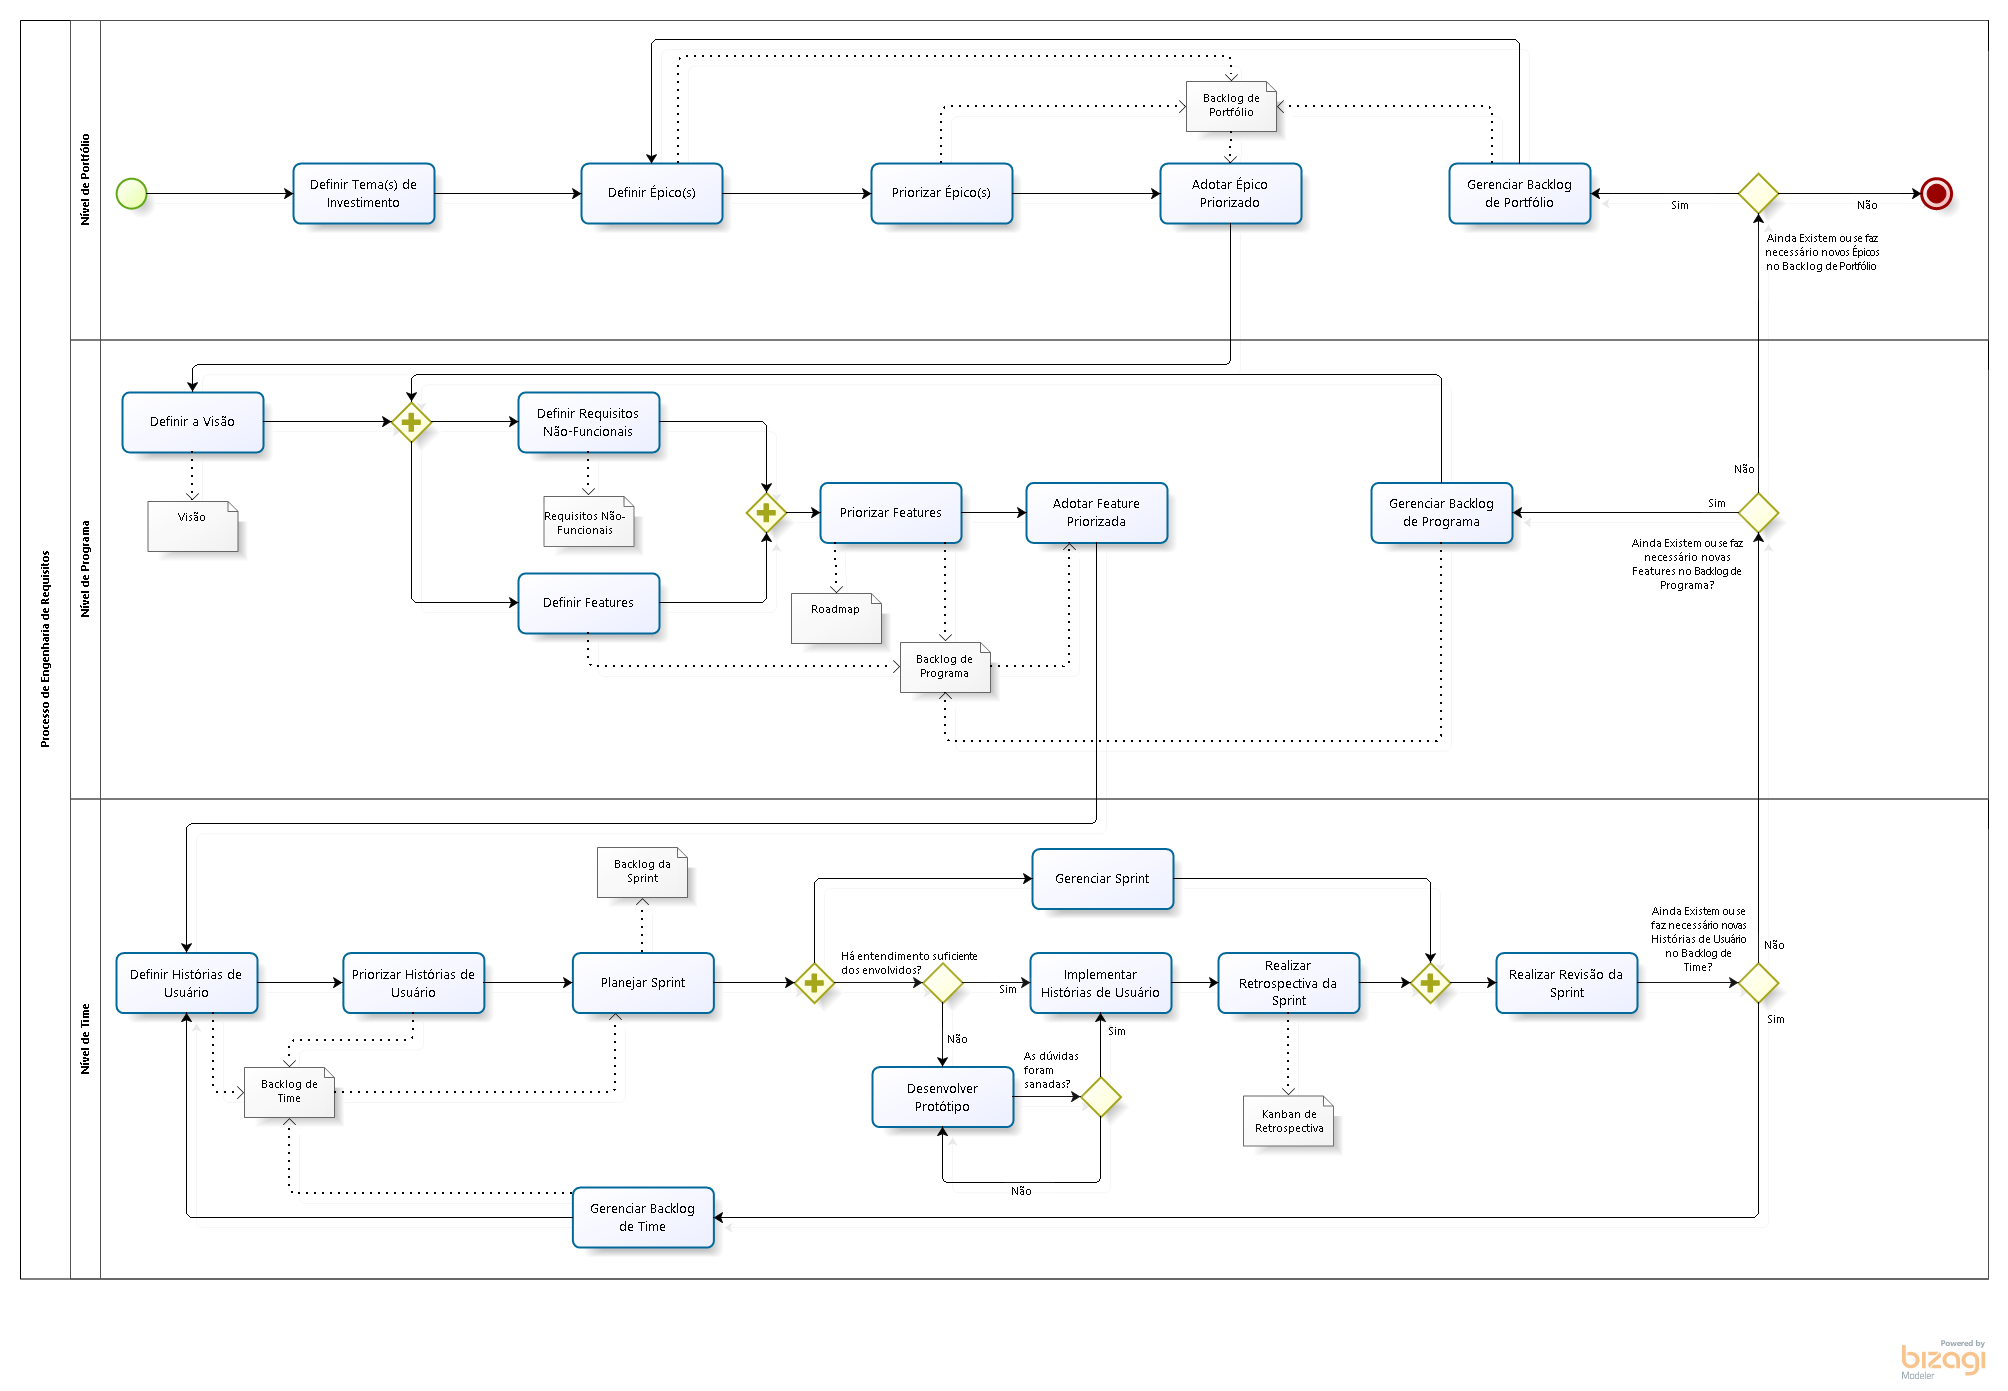
\includegraphics[scale=0.34]{processo_modelo}
				\caption[Modelo do Processo de Engenharia de Requisitos]{Modelo do Processo de Engenharia de Requisitos inspirado no SAFe \cite{safe}.}
				\label{fig:modelo_processo}
			\end{figure}
	\end{landscape}

	\section[Atividades]{Atividades}
	\label{sec:processo_atividades}
		O Processo de Engenharia de Requisitos descrito no fluxograma da Figura \ref{fig:modelo_processo} estabelece 3 níveis de atuação, 20 atividades e 7 artefatos principais.

		\subsection[Nível de Portfólio]{Nível de Portfólio}
		\label{subsec:processo_atividade_portfolio}
			De acordo com o SAFe \cite{safe}, o nível de Portfólio é o maior nível do \emph{framework}, onde os programas são alinhados pela estratégia de negócio da organização.
			\\ \indent No contexto da disciplina, aborda-se 5 atividades de Portfólio e 1 artefato principal.

			\subsubsection[Atividade: Definir Tema(s) de Investimento]{Atividade: Definir Tema(s) de Investimento}
			\label{subsubsec:processo_atividade_portfolio_definir_tema}
				\begin{itemize}
					\item{\textbf{Descrição}:
						\begin{itemize}
							\item{\textbf{SAFe}: Temas de Investimento (\emph{Strategic Themes}, em inglês) são objetivos específicos de negócio que conecta a Visão de Portfólio com a evolução da estratégia de negócio da organização;}
							\item{\textbf{Contexto do Projeto}: Conceituar itens motrizes da organização e definir Temas de Investimento, que são objetivos específicos de negócio que guiam as prioridades de investimento, assegurando que o trabalho organizado está alinhado com a estratégia de negócio da organização.}
						\end{itemize}}
					\item{\textbf{Tarefa(s)}:
						\begin{enumerate}
							\item{\textbf{Conceituar a Estratégia de Negócio}: Estabelecer a missão e valores da organização;}
							\item{\textbf{Conceituar a Análise de Competitivade}: Estabelecer maiores ameaças e áreas de oportunidade para a organização;}
							\item{\textbf{Definir Temas de Investimento}: Estabelecer objetivos da organização.}
						\end{enumerate}}
					\item{\textbf{Artefato(s) de Entrada}:
						\begin{itemize}
							\item{Não há artefatos de entrada para esta atividade.}
						\end{itemize}}
					\item{\textbf{Artefato(s) Gerado(s) e/ou Alterado(s)}:
						\begin{itemize}
							\item{\textbf{Estratégia de Negócio}: Documento descrevendo a missão e valores da organização;}
							\item{\textbf{Análise de Competitivade}: Documento descrevendo uma análise de ameaças e oportunidades para a organização;}
							\item{\textbf{Temas de Investimento}: Descrição de mais alto nível da Organização, estabelecendo os objetivos da organização.}
						\end{itemize}}
					\item{\textbf{Atividade(s) Predecessora(s)}:
						\begin{itemize}
							\item{Esta é a primeira atividade do processo.}
						\end{itemize}}
					\item{\textbf{Atividade(s) Sucessora(s)}:
						\begin{itemize}
							\item{\nameref{subsubsec:processo_atividade_portfolio_definir_epico}.}
						\end{itemize}}
				\end{itemize}

			\subsubsection[Atividade: Definir Épico(s)]{Atividade: Definir Épico(s)}
			\label{subsubsec:processo_atividade_portfolio_definir_epico}
				\begin{itemize}
					\item{\textbf{Descrição}:
						\begin{itemize}
							\item{\textbf{SAFe}: Épicos (\emph{Business Epics}, em inglês) são grandes iniciativas, tipicamente transversais ao cliente, que encapsulam novos desenvolvimentos necessários para conquistar benefícios específicos de negócio;}
							\item{\textbf{Contexto do Projeto}: Elicitar e definir Épicos, que são iniciativas de desenvolvimento que tem como objetivo entregar valor à um tema de investimento.}
						\end{itemize}}
					\item{\textbf{Tarefa(s)}:
						\begin{enumerate}
							\item{\textbf{Elicitar Épico(s) com \emph{Stakeholders}}: Estabelecer, através do uso de técnicas de elicitação (Ver Capítulo \ref{chap:elicitacao}), épicos que satisfaçam as intenções de desenvolvimento dos \emph{Stakeholders};}
							\item{\textbf{Validar Épico(s) com \emph{Stakeholders}}: Verificar se há ambiguidades ou se os épicos não estabelecem uma descrição clara da iniciativa de desenvolvimento. Aplicar modificações necessárias;}
						\end{enumerate}}
					\item{\textbf{Artefato(s) de Entrada}:
						\begin{itemize}
							\item{\textbf{Temas de Investimento}: Descrição de mais alto nível da Organização, estabelecendo os objetivos da organização.}
						\end{itemize}}
					\item{\textbf{Artefato(s) Gerado(s) e/ou Alterado(s)}:
						\begin{itemize}
							\item{\textbf{Épicos}: Descrição de iniciativas de desenvolvimento;}
							\item{\textbf{\emph{Backlog} de Portfólio}: Conjunto de Épicos.}
						\end{itemize}}
					\item{\textbf{Atividade(s) Predecessora(s)}:
						\begin{itemize}
							\item{\nameref{subsubsec:processo_atividade_portfolio_definir_tema}.}
						\end{itemize}}
					\item{\textbf{Atividade(s) Sucessora(s)}:
						\begin{itemize}
							\item{\nameref{subsubsec:processo_atividade_portfolio_priorizar_epico}.}
						\end{itemize}}
				\end{itemize}

			\subsubsection[Atividade: Priorizar Épico(s)]{Atividade: Priorizar Épico(s)}
			\label{subsubsec:processo_atividade_portfolio_priorizar_epico}
				\begin{itemize}
					\item{\textbf{Descrição}:
						\begin{itemize}
							\item{\textbf{SAFe}: Épicos (\emph{Business Epics}, em inglês) são grandes iniciativas, tipicamente transversais ao cliente, que encapsulam novos desenvolvimentos necessários para conquistar benefícios específicos de negócio;}
							\item{\textbf{Contexto do Projeto}: Ordenar Épicos em relação à sua relevância para o negócio. Épicos são iniciativas de desenvolvimento que tem como objetivo entregar valor à um tema de investimento.}
						\end{itemize}}
					\item{\textbf{Tarefa(s)}:
						\begin{enumerate}
							\item{\textbf{Definir Critérios de Avaliação com \emph{Stakeholders}}: Estabelecer pontos-chave de valores de negócio que serão utilizados para a comparação dos Épicos;}
							\item{\textbf{Priorizar Épicos com \emph{Stakeholders}}: Ordenar, de acordo com os critérios estabelecidos, os Épicos do \emph{Backlog} de Portfólio;}
						\end{enumerate}}
					\item{\textbf{Artefato(s) de Entrada}:
						\begin{itemize}
							\item{\textbf{\emph{Backlog} de Portfólio}: Conjunto de Épicos.}
						\end{itemize}}
					\item{\textbf{Artefato(s) Gerado(s) e/ou Alterado(s)}:
						\begin{itemize}
							\item{\textbf{\emph{Backlog} de Portfólio}: Conjunto de Épicos.}
						\end{itemize}}
					\item{\textbf{Atividade(s) Predecessora(s)}:
						\begin{itemize}
							\item{\nameref{subsubsec:processo_atividade_portfolio_gerenciar}, ou;}
							\item{\nameref{subsubsec:processo_atividade_portfolio_definir_epico}.}
						\end{itemize}}
					\item{\textbf{Atividade(s) Sucessora(s)}:
						\begin{itemize}
							\item{\nameref{subsubsec:processo_atividade_portfolio_adotar_epico}.}
						\end{itemize}}
				\end{itemize}

			\subsubsection[Atividade: Adotar Épico Priorizado]{Atividade: Adotar Épico Priorizado}
			\label{subsubsec:processo_atividade_portfolio_adotar_epico}
				\begin{itemize}
					\item{\textbf{Descrição}:
						\begin{itemize}
							\item{\textbf{SAFe}: Épicos (\emph{Business Epics}, em inglês) são grandes iniciativas, tipicamente transversais ao cliente, que encapsulam novos desenvolvimentos necessários para conquistar benefícios específicos de negócio;}
							\item{\textbf{Contexto do Projeto}: Escolher Épico de maior relevância para o negócio para ser desenvolvido. Épicos são iniciativas de desenvolvimento que tem como objetivo entregar valor à um tema de investimento.}
						\end{itemize}}
					\item{\textbf{Tarefa(s)}:
						\begin{enumerate}
							\item{\textbf{Confirmar Adoção com \emph{Stakeholders}}: Aprovar a escolha do épico a ser desenvolvido com os \emph{Stakeholders}.}
						\end{enumerate}}
					\item{\textbf{Artefato(s) de Entrada}:
						\begin{itemize}
							\item{\textbf{\emph{Backlog} de Portfólio}: Conjunto de Épicos;}
						\end{itemize}}
					\item{\textbf{Artefato(s) Gerado(s) e/ou Alterado(s)}:
						\begin{itemize}
							\item{Não há criação nem alteração de artefatos nessa atividade.}
						\end{itemize}}
					\item{\textbf{Atividade(s) Predecessora(s)}:
						\begin{itemize}
							\item{\nameref{subsubsec:processo_atividade_portfolio_priorizar_epico}.}
						\end{itemize}}
					\item{\textbf{Atividade(s) Sucessora(s)}:
						\begin{itemize}
							\item{\nameref{subsubsec:processo_atividade_programa_visao}.}
						\end{itemize}}
				\end{itemize}

			\subsubsection[Atividade: Gerenciar \emph{Backlog} de Portfólio]{Atividade: Gerenciar \emph{Backlog} de Portfólio}
			\label{subsubsec:processo_atividade_portfolio_gerenciar}
				\begin{itemize}
					\item{\textbf{Descrição}:
						\begin{itemize}
							\item{\textbf{SAFe}: \emph{Backlog} de Portfólio é o \emph{Backlog} de maior nível do \emph{framework}, que provê um mecanismo de armazenamento para os Épicos;}
							\item{\textbf{Contexto do Projeto}: Gerenciar o \emph{Backlog} de Portfólio, que é um conjunto de épicos armazenados.}
						\end{itemize}}
					\item{\textbf{Tarefa(s)}:
						\begin{enumerate}
							\item{\textbf{Revisar \emph{Backlog} de Portfólio com \emph{Stakeholders}}: Verificar, com o épico previamente adotado já desenvolvido, se há necessidade de novos épicos além daqueles que já estão no \emph{Backlog} de Portfólio;}
						\end{enumerate}}
					\item{\textbf{Artefato(s) de Entrada}:
						\begin{itemize}
							\item{\textbf{\emph{Backlog} de Portfólio}: Conjunto de Épicos;}
						\end{itemize}}
					\item{\textbf{Artefato(s) Gerado(s) e/ou Alterado(s)}:
						\begin{itemize}
							\item{\textbf{\emph{Backlog} de Portfólio}: Conjunto de Épicos;}
						\end{itemize}}
					\item{\textbf{Atividade(s) Predecessora(s)}:
						\begin{itemize}
							\item{\nameref{subsubsec:processo_atividade_time_revisao}, se:
							\\ Não existir Histórias de Usuário no \emph{Backlog} de time, e;
							\\ Não existir \emph{Features} no \emph{Backlog} de Programa, e;
							\\ Ainda existir Épicos no \emph{Backlog} de Portfólio ou se faz necessário criar novos Épicos.}
						\end{itemize}}
					\item{\textbf{Atividade(s) Sucessora(s)}:
						\begin{itemize}
							\item{\nameref{subsubsec:processo_atividade_portfolio_definir_epico}.}
						\end{itemize}}
				\end{itemize}

		\subsection[Nível de Programa]{Nível de Programa}
		\label{subsec:processo_atividade_programa}
			De acordo com o SAFe \cite{safe}, é no nível de Programa que os esforços dos times ágeis são alinhados e integrados para criar um maior valor às necessidades da organização e dos \emph{Stakeholders}, escalado em três construções principais: Valor, Times e \emph{Timebox}.
			\\ \indent No contexto da disciplina, onde possui apenas um time, utiliza-se apenas a construção de Valor, com o objetivo de descrever comportamentos do sistema em um nível alto de abstração através de \emph{Features} e da Visão, além do \emph{Roadmap}. Aborda-se 6 atividades de Programa e 4 artefatos principais.

			\subsubsection[Atividade: Definir a Visão]{Atividade: Definir a Visão}
			\label{subsubsec:processo_atividade_programa_visao}
				\begin{itemize}
					\item{\textbf{Descrição}:
						\begin{itemize}
							\item{\textbf{SAFe}: A Visão descreve um conjunto de soluções à serem desenvolvidas, refletindo as necessidades dos \emph{Stakeholders} e às funcionalidades propostas para atender tais necessidades;}
							\item{\textbf{Contexto do Projeto}: Definir a Visão do projeto. A Visão descreve um conjunto de soluções à serem desenvolvidas, refletindo as necessidades dos \emph{Stakeholders} e às funcionalidades propostas para atender tais necessidades.}
						\end{itemize}}
					\item{\textbf{Tarefa(s)}:
						\begin{enumerate}
							\item{\textbf{Recolher Dados do Nível de Portfólio}: Desenvolver a Visão com dados relativos aos Temas de Investimento e \emph{Backlog} de Portfólio;}
							\item{\textbf{Recolher Dados dos \emph{Stakeholders}}: Desenvolver a Visão com dados adicionais extraídos dos \emph{Stakeholders};}
							\item{\textbf{Recolher Dados da Organização}: Desenvolver a Visão com dados adicionais extraídos dos integrantes da organização;}
							\item{\textbf{Validar Visão com \emph{Stakeholders}}: Aprovar, com os \emph{Stakeholder}, a Visão.}
						\end{enumerate}}
					\item{\textbf{Artefato(s) de Entrada}:
						\begin{itemize}
							\item{\textbf{Estratégia de Negócio}: Documento descrevendo a missão e valores da organização;}
							\item{\textbf{Análise de Competitivade}: Documento descrevendo uma análise de ameaças e oportunidades para a organização;}
							\item{\textbf{Temas de Investimento}: Descrição de mais alto nível da Organização, estabelecendo os objetivos da organização;}
							\item{\textbf{\emph{Backlog} de Portfólio}: Conjunto de Épicos;}
							\item{\textbf{Dados de \emph{Stakeholders}}: Informações advindas dos \emph{Stakeholdes} à serem incrementadas na Visão, em que os \emph{Stakeholders} e/ou a Organização julgaram necessárias;}
							\item{\textbf{Dados da Organização}: Informações advindas de integrantes da organização à serem incrementadas na Visão, em que os \emph{Stakeholders} e/ou a Organização julgaram necessárias.}
						\end{itemize}}
					\item{\textbf{Artefato(s) Gerado(s) e/ou Alterado(s)}:
						\begin{itemize}
							\item{\textbf{Visão}: Documento que descreve soluções à serem desenvolvidas.}
						\end{itemize}}
					\item{\textbf{Atividade(s) Predecessora(s)}:
						\begin{itemize}
							\item{\nameref{subsubsec:processo_atividade_portfolio_adotar_epico}.}
						\end{itemize}}
					\item{\textbf{Atividade(s) Sucessora(s)}:
						\begin{itemize}
							\item{\nameref{subsubsec:processo_atividade_programa_definir_rnf}, e;}
							\item{\nameref{subsubsec:processo_atividade_programa_definir_feature}.}
						\end{itemize}}
				\end{itemize}

			\subsubsection[Atividade: Definir Requisitos Não-Funcionais]{Atividade: Definir Requisitos Não-Funcionais}
			\label{subsubsec:processo_atividade_programa_definir_rnf}
				\begin{itemize}
					\item{\textbf{Descrição}:
						\begin{itemize}
							\item{\textbf{SAFe}: Requisitos Não-Funcionais (Nonfunctional requirements, NFRs, em inglês) ou Qualidades do Sistema, descrevem atributos do sistema como: Segurança, confiabilidade, manutenibilidade e usabilidade. Também podem descrever restrições no \emph{design} do sistema;}
							\item{\textbf{Contexto do Projeto}: Elicitar e definir os Requisitos Não-Funcionais. Os Requisitos Não-Funcionais no contexto equivalem ao SAFe.}
						\end{itemize}}
					\item{\textbf{Tarefa(s)}:
						\begin{enumerate}
							\item{\textbf{Elicitar Requisitos Não-Funcionais com \emph{Stakeholders}}: Estabelecer, através do uso de técnicas de elicitação (Ver Capítulo \ref{chap:elicitacao}), requisitos não-funcionais que satisfaçam as intenções de desenvolvimento dos \emph{Stakeholders};}
							\item{\textbf{Validar Requisitos Não-Funcionais com \emph{Stakeholders}}: Verificar se há ambiguidades ou se os requisitos não-funcionais não estabelecem uma descrição clara. Aplicar modificações necessárias;}
						\end{enumerate}}
					\item{\textbf{Artefato(s) de Entrada}:
						\begin{itemize}
							\item{\textbf{Visão}: Documento que descreve soluções à serem desenvolvidas.}
						\end{itemize}}
					\item{\textbf{Artefato(s) Gerado(s) e/ou Alterado(s)}:
						\begin{itemize}
							\item{\textbf{Requisitos Não-Funcionais}: Atributos e Restrições do Sistema, anexados ao \emph{Backlog} de Portfólio, Programa e Time, comumente denominado de Restrições de \emph{Backlog}.}
						\end{itemize}}
					\item{\textbf{Atividade(s) Predecessora(s)}:
						\begin{itemize}
							\item{\nameref{subsubsec:processo_atividade_programa_visao}, ou;}
							\item{\nameref{subsubsec:processo_atividade_programa_gerenciar}.}
						\end{itemize}}
					\item{\textbf{Atividade(s) Sucessora(s)}:
						\begin{itemize}
							\item{\nameref{subsubsec:processo_atividade_programa_priorizar_feature}, se:
							\\ \nameref{subsubsec:processo_atividade_programa_definir_feature} for realizada.}
						\end{itemize}}
				\end{itemize}

			\subsubsection[Atividade: Definir \emph{Features}]{Atividade: Definir \emph{Features}}
			\label{subsubsec:processo_atividade_programa_definir_feature}
				\begin{itemize}
					\item{\textbf{Descrição}:
						\begin{itemize}
							\item{\textbf{SAFe}: \emph{Features} são funcionalidades do sistema que atendem as necessidades dos \emph{Stakeholders};}
							\item{\textbf{Contexto do Projeto}: Elicitar e definir as \emph{Features}. As \emph{Features} no contexto equivalem ao SAFe.}
						\end{itemize}}
					\item{\textbf{Tarefa(s)}:
						\begin{enumerate}
							\item{\textbf{Elicitar \emph{Features} com \emph{Stakeholders}}: Estabelecer, através do uso de técnicas de elicitação (Ver Capítulo \ref{chap:elicitacao}), \emph{features} que satisfaçam as intenções de desenvolvimento dos \emph{Stakeholders};}
							\item{\textbf{Validar \emph{Features} com \emph{Stakeholders}}: Verificar se há ambiguidades ou se as \emph{features} não estabelecem uma descrição clara. Aplicar modificações necessárias;}
						\end{enumerate}}
					\item{\textbf{Artefato(s) de Entrada}:
						\begin{itemize}
							\item{\textbf{\emph{Backlog} de Portfólio}: Conjunto de Épicos.}
						\end{itemize}}
					\item{\textbf{Artefato(s) Gerado(s) e/ou Alterado(s)}:
						\begin{itemize}
							\item{\textbf{\emph{Features}}: Descrição de funcionalidades do sistema;}
							\item{\textbf{\emph{Backlog} de Programa}: Conjunto de \emph{Features}.}
						\end{itemize}}
					\item{\textbf{Atividade(s) Predecessora(s)}:
						\begin{itemize}
							\item{\nameref{subsubsec:processo_atividade_programa_visao}, ou;}
							\item{\nameref{subsubsec:processo_atividade_programa_gerenciar}.}
						\end{itemize}}
					\item{\textbf{Atividade(s) Sucessora(s)}:
						\begin{itemize}
							\item{\nameref{subsubsec:processo_atividade_programa_priorizar_feature}, se:
							\\ \nameref{subsubsec:processo_atividade_programa_definir_rnf} for realizada.}
						\end{itemize}}
				\end{itemize}

			\subsubsection[Atividade: Priorizar \emph{Features}]{Atividade: Priorizar \emph{Features}}
			\label{subsubsec:processo_atividade_programa_priorizar_feature}
				\begin{itemize}
					\item{\textbf{Descrição}:
						\begin{itemize}
							\item{\textbf{SAFe}: \emph{Features} são funcionalidades do sistema que atendem as necessidades dos \emph{Stakeholders};}
							\item{\textbf{Contexto do Projeto}: Ordenar \emph{Features} em relação à sua relevância para o desenvolvimento do Épico. As \emph{Features} no contexto equivalem ao SAFe.}
						\end{itemize}}
					\item{\textbf{Tarefa(s)}:
						\begin{enumerate}
							\item{\textbf{Definir Critérios de Avaliação com \emph{Stakeholders}}: Estabelecer métricas de priorização que serão utilizados para a comparação das \emph{Features};}
							\item{\textbf{Priorizar \emph{Features} com \emph{Stakeholders}}: Ordenar, de acordo com os critérios estabelecidos, as \emph{Features} do \emph{Backlog} de Programa;}
							\item{\textbf{Desenvolver \emph{Roadmap}}: Estabelecer, em um fluxo temporal, as \emph{Features} à serem desenvolvidas e entregues em forma de \emph{Releases}.}
						\end{enumerate}}
					\item{\textbf{Artefato(s) de Entrada}:
						\begin{itemize}
							\item{\textbf{\emph{Backlog} de Programa}: Conjunto de \emph{Features}.}
						\end{itemize}}
					\item{\textbf{Artefato(s) Gerado(s) e/ou Alterado(s)}:
						\begin{itemize}
							\item{\textbf{\emph{Backlog} de Programa}: Conjunto de \emph{Features};}
							\item{\textbf{\emph{Roadmap}}: Fluxo temporal que descreve a ordem de desenvolvimento das \emph{Features} à serem entregues em forma de \emph{Releases}.}
						\end{itemize}}
					\item{\textbf{Atividade(s) Predecessora(s)}:
						\begin{itemize}
							\item{\nameref{subsubsec:processo_atividade_programa_definir_rnf}, e;}
							\item{\nameref{subsubsec:processo_atividade_programa_definir_feature}.}
						\end{itemize}}
					\item{\textbf{Atividade(s) Sucessora(s)}:
						\begin{itemize}
							\item{\nameref{subsubsec:processo_atividade_programa_adotar_feature}.}
						\end{itemize}}
				\end{itemize}

			\subsubsection[Atividade: Adotar \emph{Feature} Priorizada]{Atividade: Adotar \emph{Feature} Priorizada}
			\label{subsubsec:processo_atividade_programa_adotar_feature}
				\begin{itemize}
					\item{\textbf{Descrição}:
						\begin{itemize}
							\item{\textbf{SAFe}: \emph{Features} são funcionalidades do sistema que atendem as necessidades dos \emph{Stakeholders};}
							\item{\textbf{Contexto do Projeto}: Escolher \emph{Feature} de maior relevância para o Épico para ser desenvolvido. As \emph{Features} no contexto equivalem ao SAFe.}
						\end{itemize}}
					\item{\textbf{Tarefa(s)}:
						\begin{enumerate}
							\item{\textbf{Confirmar Adoção com \emph{Stakeholders}}: Aprovar a escolha da \emph{Feature} a ser desenvolvida com os \emph{Stakeholders}.}
						\end{enumerate}}
					\item{\textbf{Artefato(s) de Entrada}:
						\begin{itemize}
							\item{\textbf{\emph{Backlog} de Programa}: Conjunto de \emph{Features}.}
						\end{itemize}}
					\item{\textbf{Artefato(s) Gerado(s) e/ou Alterado(s)}:
						\begin{itemize}
							\item{Não há criação nem alteração de artefatos nessa atividade.}
						\end{itemize}}
					\item{\textbf{Atividade(s) Predecessora(s)}:
						\begin{itemize}
							\item{\nameref{subsubsec:processo_atividade_programa_priorizar_feature}.}
						\end{itemize}}
					\item{\textbf{Atividade(s) Sucessora(s)}:
						\begin{itemize}
							\item{\nameref{subsubsec:processo_atividade_time_definir_us}.}
						\end{itemize}}
				\end{itemize}

			\subsubsection[Atividade: Gerenciar \emph{Backlog} de Programa]{Atividade: Gerenciar \emph{Backlog} de Programa}
			\label{subsubsec:processo_atividade_programa_gerenciar}
				\begin{itemize}
					\item{\textbf{Descrição}:
						\begin{itemize}
							\item{\textbf{SAFe}: \emph{Backlog} de Programa é um repositório definitivo para todas as \emph{Features} do projeto;}
							\item{\textbf{Contexto do Projeto}: Gerenciar o \emph{Backlog} de Programa, que é um conjunto de \emph{Features} armazenadas.}
						\end{itemize}}
					\item{\textbf{Tarefa(s)}:
						\begin{enumerate}
							\item{\textbf{Revisar \emph{Backlog} de Programa com \emph{Stakeholders}}: Verificar, com a \emph{Feature} previamente adotada já desenvolvida, se há necessidade de novas \emph{Features} além daqueles que já estão no \emph{Backlog} de Programa;}
						\end{enumerate}}
					\item{\textbf{Artefato(s) de Entrada}:
						\begin{itemize}
							\item{\textbf{\emph{Backlog} de Programa}: Conjunto de \emph{Features};}
						\end{itemize}}
					\item{\textbf{Artefato(s) Gerado(s) e/ou Alterado(s)}:
						\begin{itemize}
							\item{\textbf{\emph{Backlog} de Programa}: Conjunto de \emph{Features};}
						\end{itemize}}
					\item{\textbf{Atividade(s) Predecessora(s)}:
						\begin{itemize}
							\item{\nameref{subsubsec:processo_atividade_time_revisao}, se:
							\\ Não existir Histórias de Usuário no \emph{Backlog} de time, e;
							\\ Ainda existir \emph{Features} no \emph{Backlog} de Programa ou se faz necessário criar novas \emph{Features.}}
						\end{itemize}}
					\item{\textbf{Atividade(s) Sucessora(s)}:
						\begin{itemize}
							\item{\nameref{subsubsec:processo_atividade_programa_definir_feature}.}
						\end{itemize}}
				\end{itemize}

		\subsection[Nível de Time]{Nível de Time}
		\label{subsec:processo_atividade_time}
			De acordo com o SAFe \cite{safe}, o Nível de Time é uma partição do Nível de Programa, pois não há possibilidades de existir Programa se não over Times. É responsabilidade no Nível de Time a definição, construção e teste de Histórias de Usuário contidas no \emph{Backlog} de Time em uma série de iterações de tempo fixo (também conhecidos como \emph{Sprints}).
			\\ \indent No contexto da disciplina, aborda-se 9 atividades de Programa e 3 artefatos principais.

			\subsubsection[Atividade: Definir Histórias de Usuário]{Atividade: Definir Histórias de Usuário}
			\label{subsubsec:processo_atividade_time_definir_us}
				\begin{itemize}
					\item{\textbf{Descrição}:
						\begin{itemize}
							\item{\textbf{SAFe}: Histórias de Usuário (User Stories, em inglês) são descrições detalhadas de uma funcionalidade à ser implementada. Cada história é curta e possui comportamente independente para que seja implementada gradualmente, agregando algum valor ao usuário. Para garantir que toda iteração disponibilize novos valores, histórias são divididos de forma que possam ser completadas em uma única iteração.}
							\item{\textbf{Contexto do Projeto}: Elicitar e definir as Histórias de Usuário. As Histórias de Usuário no contexto equivalem ao SAFe.}
						\end{itemize}}
					\item{\textbf{Tarefa(s)}:
						\begin{enumerate}
							\item{\textbf{Elicitar Histórias de Usuário com \emph{Stakeholders}}: Estabelecer, através do uso de técnicas de elicitação (Ver Capítulo \ref{chap:elicitacao}), Histórias de Usuário que satisfaçam as intenções de desenvolvimento dos \emph{Stakeholders};}
							\item{\textbf{Validar Histórias de Usuário com \emph{Stakeholders}}: Verificar se há ambiguidades ou se as Histórias de Usuário não estabelecem uma descrição clara. Aplicar modificações necessárias;}
						\end{enumerate}}
					\item{\textbf{Artefato(s) de Entrada}:
						\begin{itemize}
							\item{\textbf{\emph{Backlog} de Programa}: Conjunto de \emph{Features};}
						\end{itemize}}
					\item{\textbf{Artefato(s) Gerado(s) e/ou Alterado(s)}:
						\begin{itemize}
							\item{\textbf{\emph{Histórias de Usuário}}: Descrições detalhadas de uma funcionalidade do sistema;}
							\item{\textbf{\emph{Backlog} de Time}: Conjunto de Histórias de Usuários;}
						\end{itemize}}
					\item{\textbf{Atividade(s) Predecessora(s)}:
						\begin{itemize}
							\item{\nameref{subsubsec:processo_atividade_programa_adotar_feature}, ou;}
							\item{\nameref{subsubsec:processo_atividade_time_gerenciar}.}
						\end{itemize}}
					\item{\textbf{Atividade(s) Sucessora(s)}:
						\begin{itemize}
							\item{\nameref{subsubsec:processo_atividade_time_priorizar_us}.}
						\end{itemize}}
				\end{itemize}

			\subsubsection[Atividade: Priorizar Histórias de Usuário]{Atividade: Priorizar Histórias de Usuário}
			\label{subsubsec:processo_atividade_time_priorizar_us}
				\begin{itemize}
					\item{\textbf{Descrição}:
						\begin{itemize}
							\item{\textbf{SAFe}: Histórias de Usuário (\emph{User Stories}) são descrições detalhadas de uma funcionalidade à ser implementada. Cada história é curta e possui comportamente independente para que seja implementada gradualmente, agregando algum valor ao usuário. Para garantir que toda iteração disponibilize novos valores, histórias são divididos de forma que possam ser completadas em uma única iteração.}
							\item{\textbf{Contexto do Projeto}: Ordenar Histórias de Usuário em relação à sua relevância para o desenvolvimento da Feature. As Histórias de Usuário no contexto equivalem ao SAFe.}
						\end{itemize}}
					\item{\textbf{Tarefa(s)}:
						\begin{enumerate}
							\item{\textbf{Definir Critérios de Avaliação com \emph{Stakeholders}}: Estabelecer métricas de priorização que serão utilizados para a comparação das Histórias de Usuário;}
							\item{\textbf{Priorizar Histórias de Usuário com \emph{Stakeholders}}: Ordenar, de acordo com os critérios estabelecidos, as Histórias de Usuário do \emph{Backlog} de Time;}
						\end{enumerate}}
					\item{\textbf{Artefato(s) de Entrada}:
						\begin{itemize}
							\item{\textbf{\emph{Backlog} de Time}: Conjunto de Histórias de Usuário.}
						\end{itemize}}
					\item{\textbf{Artefato(s) Gerado(s) e/ou Alterado(s)}:
						\begin{itemize}
							\item{\textbf{\emph{Backlog} de Time}: Conjunto de Histórias de Usuário.}
						\end{itemize}}
					\item{\textbf{Atividade(s) Predecessora(s)}:
						\begin{itemize}
							\item{\nameref{subsubsec:processo_atividade_time_definir_us}.}
						\end{itemize}}
					\item{\textbf{Atividade(s) Sucessora(s)}:
						\begin{itemize}
							\item{\nameref{subsubsec:processo_atividade_time_planejar}.}
						\end{itemize}}
				\end{itemize}

			\subsubsection[Atividade: Planejar \emph{Sprint}]{Atividade: Planejar \emph{Sprint}}
			\label{subsubsec:processo_atividade_time_planejar}
				\begin{itemize}
					\item{\textbf{Descrição}:
						\begin{itemize}
							\item{\textbf{SAFe}: \emph{Sprint} é uma iteração padronizada e simples. De forma simples, uma \emph{Sprint} compreende a definição, construção e validação de incrementos em uma período de tempo fixo. A sequência é composta em planejar a iteração, estabelecer um conjunto de Histórias de Usuários e metas, desenvolver as histórias selecionadas, demonstrar o trabalho para os \emph{Stakeholders}, e realizar a retrospectiva da iteração.}
							\item{\textbf{Contexto do Projeto}: Planejar a iteração, definindo histórias de usuário à serem implementadas. \emph{Sprint} no contexto equivale ao SAFe.}
						\end{itemize}}
					\item{\textbf{Tarefa(s)}:
						\begin{enumerate}
							\item{\textbf{Popular o \emph{Backlog} da \emph{Sprint}}: Escolher Histórias de Usuário do \emph{Backlog} de Time para serem implementadas na \emph{Sprint};}
							\item{\textbf{Definir metas de \emph{Sprint}}: Estabelecer objetivos de implementação da \emph{Sprint};}
							\item{\textbf{Atribuir Tarefas aos Integrantes do Time}: Dividir as Histórias de Usuário à serem implementadas pelos desenvolvedores do time e atribuir tarefas de gerência aos integrantes.}
						\end{enumerate}}
					\item{\textbf{Artefato(s) de Entrada}:
						\begin{itemize}
							\item{\textbf{\emph{Backlog} de Time}: Conjunto de Histórias de Usuário.}
						\end{itemize}}
					\item{\textbf{Artefato(s) Gerado(s) e/ou Alterado(s)}:
						\begin{itemize}
							\item{\textbf{\emph{Backlog} da \emph{Sprint}}: Subconjunto do \emph{Backlog} de Time, com as Histórias de Usuário a serem implementadas na \emph{Sprint}.}
						\end{itemize}}
					\item{\textbf{Atividade(s) Predecessora(s)}:
						\begin{itemize}
							\item{\nameref{subsubsec:processo_atividade_time_priorizar_us}.}
						\end{itemize}}
					\item{\textbf{Atividade(s) Sucessora(s)}:
						\begin{itemize}
							\item{\nameref{subsubsec:processo_atividade_time_implementar_us}, se:
								\\ Há entendimento suficiente dos envolvidos, ou;}
							\item{\nameref{subsubsec:processo_atividade_time_prototipo}, se:
								\\ Não há entendimento suficiente dos envolvidos, e;}
							\item{\nameref{subsubsec:processo_atividade_time_gerenciar_sprint}.}
						\end{itemize}}
				\end{itemize}

			\subsubsection[Atividade: Gerenciar \emph{Sprint}]{Atividade: Gerenciar \emph{Sprint}}
			\label{subsubsec:processo_atividade_time_gerenciar_sprint}
				\begin{itemize}
					\item{\textbf{Descrição}:
						\begin{itemize}
							\item{\textbf{SAFe}: \emph{Sprint} é uma iteração padronizada e simples. De forma simples, uma \emph{Sprint} compreende a definição, construção e validação de incrementos em uma período de tempo fixo. A sequência é composta em planejar a iteração, estabelecer um conjunto de Histórias de Usuários e metas, desenvolver as histórias selecionadas, demonstrar o trabalho para os \emph{Stakeholders}, e realizar a retrospectiva da iteração.}
							\item{\textbf{Contexto do Projeto}: Gerenciar a iteração atualizando métricas e respondendo às mudanças. \emph{Sprint} no contexto equivale ao SAFe.}
						\end{itemize}}
					\item{\textbf{Tarefa(s)}:
						\begin{enumerate}
							\item{\textbf{Gerenciar o \emph{Burndown Chart}}: Criar e manter o gráfico de redução de pontos de Histórias de Usuários da \emph{Sprint};}
							\item{\textbf{Gerenciar o \emph{Velocity}}: Criar e manter o gráfico de implementação de pontos de Histórias de Usuários da \emph{Sprint};}
							\item{\textbf{Gerir Time}: Analisar e aperfeiçoar o desenvolvimento do time;}
							\item{\textbf{Responder às Mudanças}: Gerenciar mudanças e acontecimentos inesperados durante a \emph{Sprint}.}
						\end{enumerate}}
					\item{\textbf{Artefato(s) de Entrada}:
						\begin{itemize}
							\item{\textbf{\emph{Backlog} da \emph{Sprint}}: Subconjunto do \emph{Backlog} de Time, com as Histórias de Usuário a serem implementadas na \emph{Sprint}.}
						\end{itemize}}
					\item{\textbf{Artefato(s) Gerado(s) e/ou Alterado(s)}:
						\begin{itemize}
							\item{\textbf{\emph{Burndown Chart} da \emph{Sprint}}: Gráfico temporal de redução de pontos de Histórias de Usuários contidas no \emph{Backlog} da \emph{Sprint};}
							\item{\textbf{\emph{Velocity Chart} da \emph{Sprint}}: Gráfico temporal de implementação de pontos de Histórias de Usuários durante a \emph{Sprint};}
						\end{itemize}}
					\item{\textbf{Atividade(s) Predecessora(s)}:
						\begin{itemize}
							\item{\nameref{subsubsec:processo_atividade_time_planejar}.}
						\end{itemize}}
					\item{\textbf{Atividade(s) Sucessora(s)}:
						\begin{itemize}
							\item{\nameref{subsubsec:processo_atividade_time_revisao}, se:
								\\ \nameref{subsubsec:processo_atividade_time_retrospectiva} for realizada;}
						\end{itemize}}
				\end{itemize}

			\subsubsection[Atividade: Implementar Histórias de Usuário]{Atividade: Implementar Histórias de Usuário}
			\label{subsubsec:processo_atividade_time_implementar_us}
				\begin{itemize}
					\item{\textbf{Descrição}:
						\begin{itemize}
							\item{\textbf{SAFe}: Histórias de Usuário (\emph{User Stories}) são descrições detalhadas de uma funcionalidade à ser implementada. Cada história é curta e possui comportamente independente para que seja implementada gradualmente, agregando algum valor ao usuário. Para garantir que toda iteração disponibilize novos valores, histórias são divididos de forma que possam ser completadas em uma única iteração.}
							\item{\textbf{Contexto do Projeto}: Desenvolver Histórias de Usuário de acordo com os critérios estabelecidos durante o planejamento da \emph{Sprint}. As Histórias de Usuário no contexto equivalem ao SAFe.}
						\end{itemize}}
					\item{\textbf{Tarefa(s)}:
						\begin{enumerate}
							\item{\textbf{Desenvolver Histórias de Usuário};}
							\item{\textbf{Verificar Funcionalidades Desenvolvidas}: Apresentar ao time as funcionalidades desenvolvidas, com o objetivo de encontrar falhas e/ou incoerências. Aplicar modificações, se necessário;}
							\item{\textbf{Validar Funcionalidades Desenvolvidas com \emph{Stakeholders}}: Apresentar ao \emph{Product Owner} e/ou outros \emph{Stakeholders} de relevância, o conjunto de funcionalidades desenvolvido, com o objetivo de validar o desenvolvimento. Aplicar modificações, se necessário;}
						\end{enumerate}}
					\item{\textbf{Artefato(s) de Entrada}:
						\begin{itemize}
							\item{\textbf{\emph{Backlog} da \emph{Sprint}}: Subconjunto do \emph{Backlog} de Time, com as Histórias de Usuário a serem implementadas na \emph{Sprint}.}
						\end{itemize}}
					\item{\textbf{Artefato(s) Gerado(s) e/ou Alterado(s)}:
						\begin{itemize}
							\item{\textbf{Incremento Funcional (\emph{Build} ou \emph{Release})}: Conjunto de funcionalidades implementadas durante uma \emph{Sprint};}
						\end{itemize}}
					\item{\textbf{Atividade(s) Predecessora(s)}:
						\begin{itemize}
							\item{\nameref{subsubsec:processo_atividade_time_planejar}, se:
								\\ Há entendimento suficiente dos envolvidos, ou;}
							\item{\nameref{subsubsec:processo_atividade_time_prototipo}, se:
								\\ As dúvidas foram sanadas.}
						\end{itemize}}
					\item{\textbf{Atividade(s) Sucessora(s)}:
						\begin{itemize}
							\item{\nameref{subsubsec:processo_atividade_time_retrospectiva}.}
						\end{itemize}}
				\end{itemize}

			\subsubsection[Atividade: Desenvolver Protótipo]{Atividade: Desenvolver Protótipo}
			\label{subsubsec:processo_atividade_time_prototipo}
				\begin{itemize}
					\item{\textbf{Descrição}:
						\begin{itemize}
							\item{\textbf{Definição de Prototipar}: Criar um demonstrativo de um sistema novo. Prototipação é essencial para tornar claro informações de requisitos. O \emph{design} do sistema (especificações funcionais) deve ser finalizada antes do sistema ser construída. Enquanto para algumas pessoas pode estar claro a imagem dos requisitos, para outros podem não estar. \cite{pcmag}}
							\item{\textbf{Contexto do Projeto}: Desenvolver protótipo(s) com o objetivo de tornar claro a intenção de uma ou mais Histórias de Usuário. As Histórias de Usuário no contexto equivalem ao SAFe.}
						\end{itemize}}
					\item{\textbf{Tarefa(s)}:
						\begin{enumerate}
							\item{\textbf{Definir Contexto de Prototipação}: Descobrir pontos não compreendidos dos envolvidos e planejar a prototipação dos mesmos;}
							\item{\textbf{Desenvolver Protótipo(s)}: Desenvolver, de forma simples, um protótipo funcional que torna claro pontos não compreendidos dos envolvidos;}
							\item{\textbf{Apresentar Protótipo(s)}: Apresentar aos envolvidos o(s) protótipo(s) desenvolvido(s). Aplicar modificações, se necessário.}
						\end{enumerate}}
					\item{\textbf{Artefato(s) de Entrada}:
						\begin{itemize}
							\item{\textbf{\emph{Backlog} da \emph{Sprint}}: Subconjunto do \emph{Backlog} de Time, com as Histórias de Usuário a serem implementadas na \emph{Sprint}.}
						\end{itemize}}
					\item{\textbf{Artefato(s) Gerado(s) e/ou Alterado(s)}:
						\begin{itemize}
							\item{\textbf{Protótipo}: Demonstrativo funcional;}
						\end{itemize}}
					\item{\textbf{Atividade(s) Predecessora(s)}:
						\begin{itemize}
							\item{\nameref{subsubsec:processo_atividade_time_planejar}, se:
								\\ Não há entendimento suficiente dos envolvidos, ou;}
							\item{\nameref{subsubsec:processo_atividade_time_prototipo}, se:
								\\ As dúvidas não foram sanadas.}
						\end{itemize}}
					\item{\textbf{Atividade(s) Sucessora(s)}:
						\begin{itemize}
							\item{\nameref{subsubsec:processo_atividade_time_implementar_us}, se:
								\\ As dúvidas foram sanadas.}
						\end{itemize}}
				\end{itemize}

			\subsubsection[Atividade: Realizar Retrospectiva da \emph{Sprint}]{Atividade: Realizar Retrospectiva da \emph{Sprint}}
			\label{subsubsec:processo_atividade_time_retrospectiva}
				\begin{itemize}
					\item{\textbf{Descrição}:
						\begin{itemize}
							\item{\textbf{SAFe}: Ao fim de cada iteração, os membros do time se reunem para a retrospectiva, aonde os membros discutem suas práticas e identifica melhorias. O tempo estabelecido é de uma hora ou menos, cada esforço de retrospectiva é voltado para descobrir \textbf{o que ocorreu bem}, \textbf{o que não ocorreu bem} e o que o time pode \textbf{fazer melhor da próxima vez}}
						\end{itemize}}
					\item{\textbf{Tarefa(s)}:
						\begin{enumerate}
							\item{\textbf{Discutir Aspectos Quantitativos}: Metas, entregas, revisões das métricas de perfomance;}
							\item{\textbf{Discutir Aspectos Qualitativos}: As práticas do time, desafios enfrentados. Caso problemas sejam identificados, se faz necessário descobrir a causa raíz e a discussão de ações corretivas.}
						\end{enumerate}}
					\item{\textbf{Artefato(s) de Entrada}:
						\begin{itemize}
							\item{\textbf{\emph{Backlog} da \emph{Sprint}}: Subconjunto do \emph{Backlog} de Time, com as Histórias de Usuário a serem implementadas na \emph{Sprint}.}
							\item{\textbf{Incremento Funcional (\emph{Build} ou \emph{Release})}: Conjunto de funcionalidades implementadas durante uma \emph{Sprint};}
							\item{\textbf{Pauta da Reunião de Retrospectiva}: Uma agenda simples de pontos à serem discutidos durante a retrospectiva.}
						\end{itemize}}
					\item{\textbf{Artefato(s) Gerado(s) e/ou Alterado(s)}:
						\begin{itemize}
							\item{\textbf{Ata da Retrospectiva}: Resumo da discussão ocorrida na retrospectiva.}
						\end{itemize}}
					\item{\textbf{Atividade(s) Predecessora(s)}:
						\begin{itemize}
							\item{\nameref{subsubsec:processo_atividade_time_implementar_us}.}
						\end{itemize}}
					\item{\textbf{Atividade(s) Sucessora(s)}:
						\begin{itemize}
							\item{\nameref{subsubsec:processo_atividade_time_revisao}.}
						\end{itemize}}
				\end{itemize}

			\subsubsection[Atividade: Realizar Revisão da \emph{Sprint}]{Atividade: Realizar Revisão da \emph{Sprint}}
			\label{subsubsec:processo_atividade_time_revisao}
				\begin{itemize}
					\item{\textbf{Descrição}:
						\begin{itemize}
							\item{\textbf{Revisão da \emph{Sprint} no Contexto do Scrum}: Durante a Revisão da \emph{Sprint}, o time e as partes interessadas colaboram sobre o que acabou de ser feito. Baseados nisso e em mudanças no \emph{Backlog} do Produto feitas durante a \emph{Sprint}, eles colaboram sobre quais são as próximas coisas que podem ser feitas. Essa é uma reunião informal, com a apresentação da funcionalidade, que tem a intenção de promover a colaboração sobre o que fazer em seguida \cite{guiadoscrum};}
						\end{itemize}}
					\item{\textbf{Tarefa(s)}:
						\begin{enumerate}
							\item{\textbf{Identificar Desenvolvimentos}: Evidenciar o que foi feito e o que não foi feito;}
							\item{\textbf{Apresentar Desenvolvimentos}: Apresentar o conjunto de funcionalidades desenvolvido;}
							\item{\textbf{Discutir Andamento do Projeto}: Estudar \emph{Backlog} de Time no contexto total do projeto, realizar projeções de datas de conclusão prováveis;}
							\item{\textbf{Concluir Revisão da \emph{Sprint}}: Identificar o que foi discutido e estabelecer diretrizes para a próxima \emph{Sprint}.}
						\end{enumerate}}
					\item{\textbf{Artefato(s) de Entrada}:
						\begin{itemize}
							\item{\textbf{\emph{Backlog} da \emph{Sprint}}: Subconjunto do \emph{Backlog} de Time, com as Histórias de Usuário a serem implementadas na \emph{Sprint};}
							\item{\textbf{\emph{Backlog} de Time}: Conjunto de Histórias de Usuário;}
							\item{\textbf{\emph{Backlog} de Programa}: Conjunto de \emph{Features};}
							\item{\textbf{Incremento Funcional (\emph{Build} ou \emph{Release})}: Conjunto de funcionalidades implementadas durante uma \emph{Sprint};}
							\item{\textbf{Pauta da Reunião de Revisão de \emph{Sprint}}: Uma agenda simples de pontos à serem discutidos durante a revisão de \emph{Sprint}.}
						\end{itemize}}
					\item{\textbf{Artefato(s) Gerado(s) e/ou Alterado(s)}:
						\begin{itemize}
							\item{\textbf{Ata da Revisão de \emph{Sprint}}: Resumo da discussão ocorrida na revisão de \emph{Sprint}.}
						\end{itemize}}
					\item{\textbf{Atividade(s) Predecessora(s)}:
						\begin{itemize}
							\item{\nameref{subsubsec:processo_atividade_time_retrospectiva}.}
						\end{itemize}}
					\item{\textbf{Atividade(s) Sucessora(s)}:
						\begin{itemize}
							\item{\nameref{subsubsec:processo_atividade_time_gerenciar}, se:
								\\ Ainda existir Histórias de Usuário no \emph{Backlog} de Time ou se faz necessário criar novas Histórias de Usuário, ou;}
							\item{\nameref{subsubsec:processo_atividade_programa_gerenciar}, se:
								\\ Não existir Histórias de Usuário no \emph{Backlog} de time, e;
								\\ Ainda existir \emph{Features} no \emph{Backlog} de Programa ou se faz necessário criar novas \emph{Features}, ou;}
							\item{\nameref{subsubsec:processo_atividade_portfolio_gerenciar}, se:
								\\ Não existir Histórias de Usuário no \emph{Backlog} de time, e;
								\\ Não existir \emph{Features} no \emph{Backlog} de Programa, e;
								\\ Ainda existir Épicos no \emph{Backlog} de Portfólio ou se faz necessário criar novos Épicos, ou;}
							\item{Evento Determinante de Fim: Encerrar o Processo, se:
								\\ Não existir Histórias de Usuário no \emph{Backlog} de time, e;
								\\ Não existir \emph{Features} no \emph{Backlog} de Programa, e;
								\\ Não existir Épicos no \emph{Backlog} de Portfólio.}
						\end{itemize}}
				\end{itemize}

			\subsubsection[Atividade: Gerenciar \emph{Backlog} de Time]{Atividade: Gerenciar \emph{Backlog} de Time}
			\label{subsubsec:processo_atividade_time_gerenciar}
				\begin{itemize}
					\item{\textbf{Descrição}:
						\begin{itemize}
							\item{\textbf{SAFe}: \emph{Backlog} de Time representa uma coleção de tudo que o time precisa fazer para avançar sua parcela de solução do sistema. Pode conter histórias de usuário, \emph{features} futuras, histórias técnicas, trabalho de infraestrutura, refatorações, e qualquer outra coisa que o time precise fazer;}
							\item{\textbf{Contexto do Projeto}: Gerenciar o \emph{Backlog} de Time, que é um conjunto de Histórias de Usuário armazenados.}
						\end{itemize}}
					\item{\textbf{Tarefa(s)}:
						\begin{enumerate}
							\item{\textbf{Revisar \emph{Backlog} de Time com \emph{Stakeholders}}: Verificar, com as Histórias de Usuário previamente adotados já desenvolvidos, se há necessidade de novas Histórias de Usuário além daqueles que já estão no \emph{Backlog} de Time;}
						\end{enumerate}}
					\item{\textbf{Artefato(s) de Entrada}:
						\begin{itemize}
							\item{\textbf{\emph{Backlog} de Time}: Conjunto de Histórias de Usuário.}
						\end{itemize}}
					\item{\textbf{Artefato(s) Gerado(s) e/ou Alterado(s)}:
						\begin{itemize}
							\item{\textbf{\emph{Backlog} de Time}: Conjunto de Histórias de Usuário.}
						\end{itemize}}
					\item{\textbf{Atividade(s) Predecessora(s)}:
						\begin{itemize}
							\item{\nameref{subsubsec:processo_atividade_time_revisao}, se:
								\\ Ainda existir Histórias de Usuário no \emph{Backlog} de Time ou se faz necessário criar novas Histórias de Usuário.}
						\end{itemize}}
					\item{\textbf{Atividade(s) Sucessora(s)}:
						\begin{itemize}
							\item{\nameref{subsubsec:processo_atividade_time_definir_us}.}
						\end{itemize}}
				\end{itemize}